
\section{Phase transitions in equilibrium}
\subsection{Motivation}

Phase is a distinct state of matter which can be described by an "order parameter". We'll focus on isotropic polar phase transition. In this case the order parameter is the polarization \( \vec{p}== \langle\hat n\rangle\) where $\hat n$ is the unit vector of the particles' direction. 

\paragraph{Phase transition}in certain areas of physics we see systems which aren't ordered at high temperatures but become ordered at low temperatures. Why? A competition between energy and entropy (Free energy being $F=U-TS$). The temperature at which order emerges is called the critical temperature, marked $T_C$ and the change in the system is called a phase transition.

\begin{figure}[!htb]
	\centering
  	\includegraphics[width=0.5\textwidth]{images/polarvsisotropic.png}
  	\caption{Polar and Isotropic ordering of matter.}
\end{figure}

\subsection{Physical description}

We'll assume free energy of the following form:

\begin{equation}
	F(T,N,\psi)=F_0(T,N)+F_\psi(T,N,\psi)
\end{equation}

where $\psi$ is the order parameter. $\psi$ is not a conserved quantity but rather a degree of freedom of the system (in contrast to the number of particles, for example). Therefore under equilibruim we find

\begin{equation}
	F_{eq}(T,N,\psi) = F_0(T,N)+F_\psi(T,N,\psi_{eq})
\end{equation}

and the equilibrium value is determined by

\begin{equation}
	\left.\diffp{F_\psi}{\psi}\right|_{\psi=\psi_{eq}}=0
\end{equation}

and the following is true:

\begin{align}
	\psi_{eq}(T>T_C) &= 0\\
	\psi_{eq}(T<T_C) &\neq 0
\end{align}

We'll focus on phase transition of 2nd order, for which the order parameter changes continuously, thus $\psi_{eq}(T=T_C)=0$. Otherwise the phase transition is of first order.

\subsection{Landau Theory of Phase Transitions}

The theory was developed by Lev Landau, for which he earned the Nobel Prize in Physics in 1962. It states that close to the critical temperature $T_C$ the physics of phase transitions is universal. For a phase transition of 2nd order, we will write $F_\psi$ in a phenomenological form as a Taylor series expansion:

\begin{equation}
	F_\psi = \frac{a}{2}\psi^2+\frac{b}{4}\psi^4
\end{equation}

The terms being of even powers because we don't care about directions. The quadratic term's coefficient is of the form

\begin{equation}
	a=a_0\cdot\frac{T-T_C}{T_C}
\end{equation}

Where $a_0>0$. This quantifies the competition between energy (which wins at $T<T_C$) and entropy (which wins at $T>T_C$. The parameter $b>0$ ensures stability: $\psi_{eq}$ receives finite values and does not approach infinity.

\begin{figure}[!htb]
	\centering
	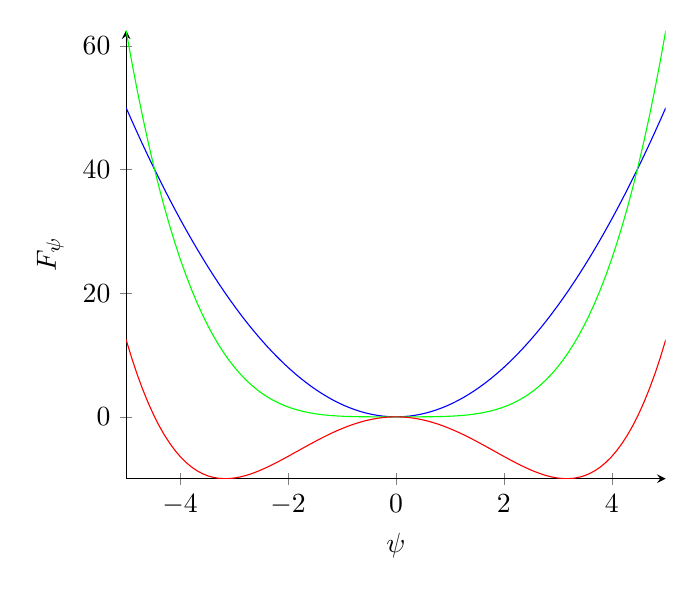
\begin{tikzpicture}
		\begin{axis}[
						axis lines=left,
						xlabel = \(\psi\),
						ylabel = {\(F_\psi\)}
					]
			\addplot[
				domain=-5:5,
				samples=100,
				color=blue
			]{2*x^2};
			\addplot[
				domain=-5:5,
				samples=100,
				color=green
			]{0.1*x^4};
			\addplot[
				domain=-5:5,
				samples=100,
				color=red
			]{0.1*x^4-2*x^2};
		\end{axis}
	\end{tikzpicture}
	\caption{The graphs for the functions $2x^2$ (blue), $0.1x^4$ (green) and $0.1x^4-2x^2$ (red).}
\end{figure}


Because of a's sign, we find $\psi_{eq}\neq0$ for $T<T_C$. Explicitly:

\begin{equation}
	0=\left.\diffp{F}{\psi}\right|_{\psi=\psi_{eq}}=a\psi_{eq}+b\psi_{eq}^3=b\psi_{eq}\left(\psi_{eq}^2+\frac{a}{b}\right)
\end{equation}

therefore

\begin{equation}\label{solution_psi_eq_ch1}
	\psi_{eq} = 0, \pm \sqrt{\frac{a_o}{b}\cdot\frac{T-T_C}{T_C}}
\end{equation}

\begin{figure}[!htb]
	\centering
	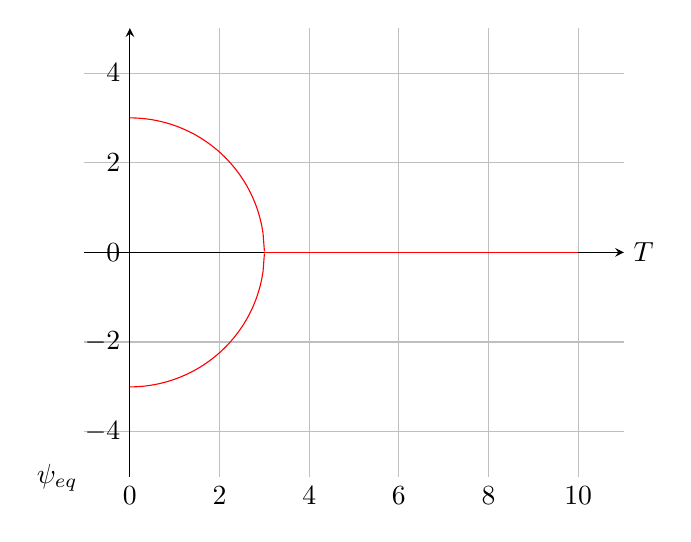
\begin{tikzpicture}
		\begin{axis}[
			axis lines = center,
			axis equal=true,
			xmin=0,
			xmax=10,
			ymin=-5,
			ymax=5,
			xlabel=\(T\),
			ylabel={$\psi_{eq}$},
			xlabel style={
            anchor=west,
        },
        ylabel style={
            anchor=north,
            shift={(0,-1.45 -| {axis description cs:-0.05,-0})}
        },
        grid=major,
        xticklabel style={
            shift={(0,0 |- {axis description cs:0,-1})}
        },
        tickwidth=0pt,
        hide obscured x ticks=false,
        hide obscured y ticks=false
		]
		\addplot[domain=0:3, red, samples=100]{sqrt(9-x^2)};
		\addplot[domain=0:3, red, samples=100]{-sqrt(9-x^2)};
		\addplot[domain=3:10, red]{0};
		\end{axis}
	\end{tikzpicture}
	\caption{The possible solutions from equation \ref{solution_psi_eq_ch1}.}
\end{figure}

There is no distinction between the positive and negative sign. Either can be chosen arbitrarily (spontaneous symmetry break). There will be a preference given an external field which will add an element of the form $-h\psi$ to the free energy.

\newpage

\subsubsection{Where the parameter $a$ comes from}

We'll assume a simple model of polarisation with energy 

\begin{equation}
	U=-\sum\limits_{i,j \;\; neighbors}un_\alpha^in_\alpha^j \;\;,\;\; u>0
\end{equation}

The energy is lower when i,j point in the same direction. Using mean field approximation the internal energy is

\begin{equation}
	U=\frac{u}{2}\sum\limits_{i,j}\langle n_\alpha^i\rangle\cdot\langle n_\alpha^j\rangle = -\frac{u}{2}NZp_\alpha^2
\end{equation}

where $p_\alpha=\langle n_\alpha\rangle$, N is the number of particles, and Z the number of close neighbors. As for the entropy, we can find from a taylor expansion

\begin{equation}
	S=S(p=0)-\alpha Np^2
\end{equation}

and summing it up we find

\begin{equation}
	F=U-TS=N\left(\alpha T-\frac{u}{2}Z\right)p^2=a_0\cdot\frac{T-T_C}{T_C}p^2
\end{equation}

where 

\begin{align}
	T_C=\frac{uZ}{2\alpha} && a_0=\alpha NT_C
\end{align}

If instead of the vector $n_\alpha$ there is spin ($\pm$) then we find a similar result in the mean field framework. This model is called the Ising model, one of the most basic and useful models in statistical mechanics.

\subsubsection{A dynamical description of the phase transition}

We described the phase transition from the free energy but we can also describe it from dynamics. For a non-conserved order parameter we can write the dynamics as follows:

\begin{equation}
	\dot\psi=-\Gamma_\psi\diffp{F}{\psi} \;\;,\;\; \Gamma_\psi>0
\end{equation}

the idea being that the dynamics guarantee that the free energy only gets smaller (the total entropy grows). We can see this using the chain rule:

\begin{align}
	\dot F &= \diffp{F}{\psi}\dot\psi=-\Gamma_\psi\left(\diffp{F}{\psi}\right)^2<0
\end{align}

this dynamics is called Model A (and often appears with a "noise" parameter). We'll insert F and find:

\begin{equation}
	\dot p = -\Gamma_p(ap+bp^3)
\end{equation}

the fixed points are $\diffp{F}{p}=0$, the extremums of the free energy. The stability of the solution is determined in phase space.

\begin{figure}[!htb]
	\centering
	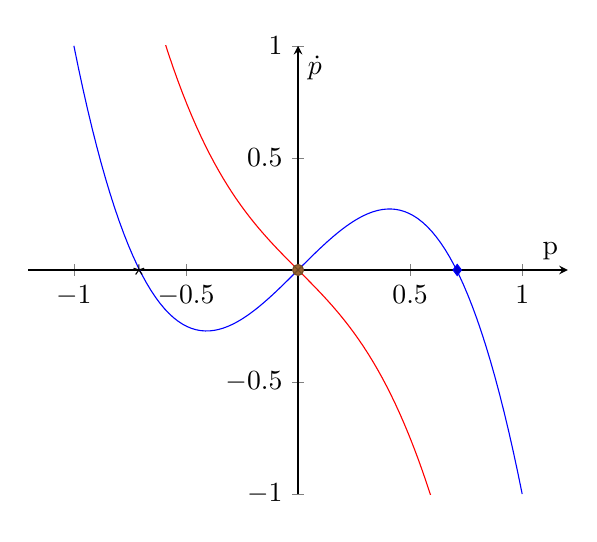
\begin{tikzpicture}
		\begin{axis}[axis lines = center,axis equal=true, xmin=-1, xmax=1, ymin=-1, ymax=1, xlabel=p, ylabel=$\dot p$]
			\plot[domain=-1:1, blue, samples=100]{x-2*x^3};
			\addplot[domain=-1:1, red, samples=100, ]{-x-2*x^3};
			\addplot coordinates{(0,0)};
			\addplot coordinates{(-0.71,0)};
			\addplot coordinates{(0.71,0)};
		\end{axis}
	\end{tikzpicture}
	\caption{The graphs of $f(x)=x-2x^3$ (blue) and $g(x)=-x-2x^3$ (red). The positive and negative points marked on the x axis are stable points of equilibrium for $f(x).$ The point marked at (0,0) is a stable point for $g(x)$ but an unstable one for $f(x).$}
\end{figure}

in the language of dynamical systems, a phase transition is called a bifurcation. This approach is useful for out of equilibrium systems, for which we can't write down a free energy. Later on in the course, we'll come across dynamical equations of a similar form.

In general dynamical systems, when a function F whose derivative is strictly non-positive with a finite minimum exists (like free energy), then it's called a Lyapunov function.

\subsection{Spatial Dependance: The Ginsburg-Landau Theory}

We saw that the direction of $\vec p\relax$ is arbitrary, in practice different areas of the system will initially develop order in different directions. For simplicity, we'll assume \( \vec p == p \hat y \relax\) where \( p \) can be either positive or negative. We'll look at the case where $ \vec p\relax $ points down at \( x\rightarrow - \infty \) and up at \( x\rightarrow\infty \). 

\begin{figure}[!htb]
	\centering\includegraphics[width=0.5\textwidth]{images/phasetransition_arrows}
	\caption{A smooth phase transition with Domain Wall $\xi$.}
\end{figure}

\newpage
\hfill\break

\begin{figure}[!htb]
	\centering\includegraphics[width=0.5\textwidth]{images/transitionarea}
	\caption{A smooth phase transition with Domain Wall $\xi$.}
\end{figure}

We'll find a finite range around 0 of width $\rchi$ in which $\abs{\vec p} \neq p_{eq}$. This region is called the Domain Wall. To quantify the cost to change $\vec p\relax$ in space we'll write the density of free energy per length unit:

\begin{equation}
	F[p]=\int\dd xf=\int\dd x\left(\frac{a}{2}p^2+\frac{b}{4}p^4+\frac{k}{2}p'^2\right)
\end{equation} 

where $k>0$. The last element quantifies the cost to change p. In higher dimensions we'll have $(\vec\nabla p)^2$. Why is it like this? The cost comes from the gradient, and given there is no preferred direction, a positive and negative change should cost the same.
